\section{Regularization}


% -----------------------------------------------------------------------------
\begin{frame}\frametitle{Regularization}
	\begin{block}{Risk function}
		\begin{equation*}
			R_{[\vec{w}]} = \underbrace{ E_{[\vec{w}]}^T }_{
					\substack{\text{training} \\ \text{error}}}
				+ \underbrace{ \lambda E_{[\vec{w}]}^R }_{
					\substack{\text{regularization} \\ \text{term}}}
				\eqexcl \min_{\vec w}
		\end{equation*}
		\begin{itemize}
			\item $E^R_{[\vec w]}:$ prior knowledge of solution
			\item $\lambda:$ regularization parameter 
		\end{itemize}
	\end{block}
	
	\begin{center}
		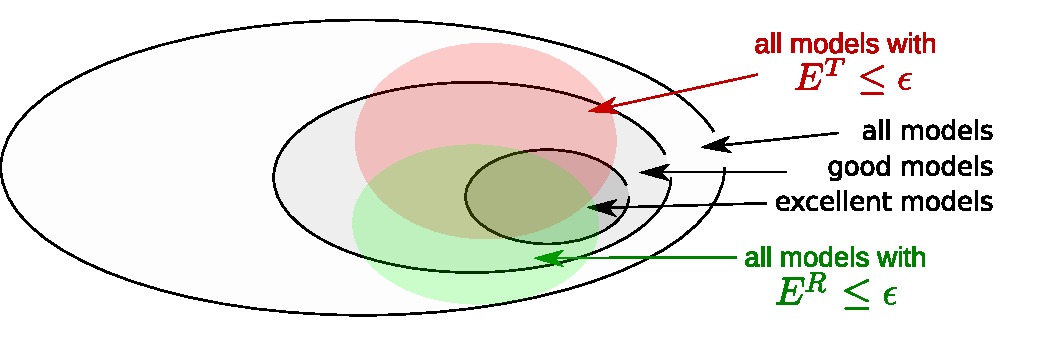
\includegraphics[width=10cm]{img/ModelSelection_models_v2.pdf}
	\end{center}
\end{frame}

\subsection{L2 regularization: weight decay}

% -----------------------------------------------------------------------------
\begin{frame}\frametitle{Regularization example: weight decay}


	\begin{center}
		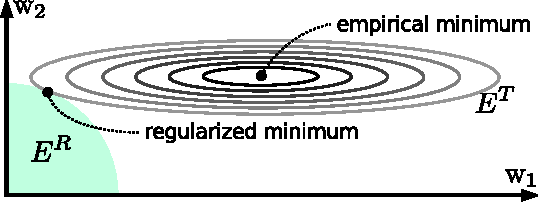
\includegraphics[width=7cm]{img/empirical_vs_regularized}
	\end{center}
	
	\begin{equation}
		E_{[\vec{w}]}^R \;=\; \frac{1}{2} \sum_{(i, j, v', v)} 
			\big( {w}_{ij}^{v'v} \big)^2 = \frac{1}{2} \vec w^\top \vec w
	\end{equation}
	
	%\only<3>{
	\begin{block}{Minimization of $R_{[\vec w]}$ through gradient descent}
		\begin{equation}
			\Delta \mathrm{w}_{ij}^{v'v} \;\sim\; 
				-\frac{\partial R_{[\vec w]}}{\partial {w}_{ij}^{v'v}}
			\;=\; - \underbrace{\frac{\partial E^T_{[\vec w]}}%
				{\partial {w}_{ij}^{v'v}}}_{
				\substack{\text{e.g. via} \\ \text{backprop}}}
			\;\;-\;\; \underbrace{\lambda {w}_{ij}^{v'v}}_{
				\substack{\text{decay} \\ \text{term}}}
		\end{equation}
	\end{block}
	%}
	
\end{frame}


\begin{frame}

$L_2$ regularization cost:
\begin{equation}
E^R_{[\vec w]} := \frac{1}{2} \sum_{(i, j, v', v)} 
			\big( \mathrm{w}_{ij}^{v'v} \big)^2 = \frac{1}{2} \lVert \vec w \rVert_2^2 = \frac{1}{2} \vec w^\top \vec w 
\end{equation}
\renewcommand{\CancelColor}{\color{gray}}

\only<1>{
Computing individual components of the gradient vector:

	\begin{align}
		\frac{\partial{E_{[\vec{w}]}^R}}{\partial {w}_{ij}^{v'v}}
		\;&=\; \frac{1}{2} \sum_{(i, j, v', v)} \frac{\partial}{\partial {w}_{ij}^{v'v}} \big( {w}_{ij}^{v'v} \big)^2\\
		\;&=\; \frac{1}{2} \sum_{(i, j, v', v)} 0 + \ldots + \frac{\partial}{\partial {w}_{ij}^{v'v}} \big( {w}_{ij}^{v'v} \big)^2 + \ldots + 0
		\;=\; \frac{1}{\cancel{2}} \; \cancel{2} \; {w}_{ij}^{v'v}
	\end{align}
}
\only<2>{
Using vector notation to compute the gradient:

\begin{equation}
\frac{\partial}{\partial \vec w} E^R_{[\vec w]} = \frac{1}{\wcancel{2}} \cdot \wcancel{2} \cdot \vec w = \vec w
\end{equation}
}

The regularized cost function:

\begin{equation}
	R_{[\vec{w}]} = \underbrace{ E_{[\vec{w}]}^T }_{
			\substack{\text{training} \\ \text{error} \\ \text{e.g. quadratic cost}}}
		+ \underbrace{ \lambda E_{[\vec{w}]}^R }_{
			\substack{\text{regularization} \\ \text{term}}}
		\eqexcl \min_{\vec w}
\end{equation}

where 
\begin{itemize}
	\item $E^R \; \corresponds \; $ prior knowledge of solution
	\item $\lambda:$ regularization parameter 
\end{itemize}

\end{frame}

\subsubsection{Regularized linear neuron for regression: analytical solution}

\begin{frame}

\slidesonly{
\begin{equation}
	R_{[\vec{w}]} = \underbrace{ E_{[\vec{w}]}^T }_{
			\substack{\text{training} \\ \text{error} \\ \text{e.g. quadratic cost}}}
		+ \underbrace{ \lambda E_{[\vec{w}]}^R }_{
			\substack{\text{regularization} \\ \text{term}}}
		\eqexcl \min_{\vec w}
\end{equation}
}
Gradient:

\begin{align}
\vec g^R :=  \frac{\partial}{\partial \vec w} R_{[\vec w]}
&= \frac{\partial}{\partial \vec w} E^T_{[\vec w]} + \frac{\partial}{\partial \vec w} E^R_{[\vec w]}\\
&= \frac{1}{p} \left(\, \vec X \, \vec X^\top \vec w - \vec X\, \vec y_{\text{True}}^\top \right) + \vec I_N \, \lambda \, \vec w\\[2mm]
\iff& \quad \vec X \, \vec X^\top \vec w - \vec X\, \vec y_{\text{True}}^\top + p \lambda \, \vec I_N \,  \vec w \eqexcl \vec 0\\[2mm]
\vec w^* &=  {\underbrace{
\left(\, \vec X \, \vec X^\top + p \lambda \, \vec I_N \,  \right)
}_{
\substack{
\text{positive definite and}\\
\text{therefore invertible}\\
}
}
}^{-1} \vec X \, \vec y_{\mathrm{True}}^{\top}
\end{align}

\end{frame}

\subsection{L1 regularization}

% -----------------------------------------------------------------------------
\begin{frame}\frametitle{\subsecname}

	\begin{equation}
		E^R_{[\vec w]} = \sum\limits_{(i, j, v', v)} {|w_{ij}^{v'v}|}^1
	\end{equation}
	
	\begin{center}
		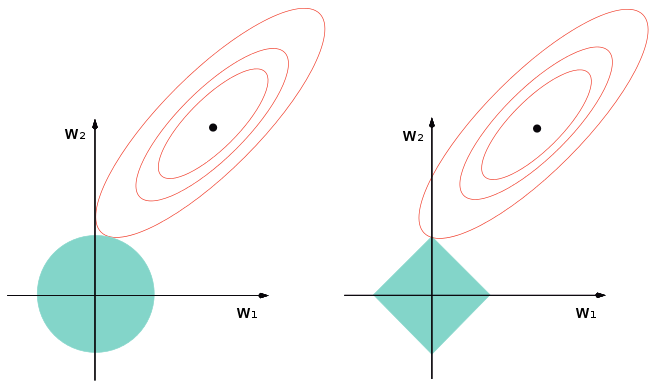
\includegraphics[width=7cm]{img/RegularizationTypesIntersect_clean.png} \\[-2mm]
		{ \footnotesize $L_2$ {\em weight decay}
			\hspace{1cm} $L_1$ {\em lasso}\hspace{1cm} $ $}
	\end{center}
	
	``Lasso'' stands for ``\textbf{l}east \textbf{a}bsolute \textbf{s}hrinkage and \textbf{s}election \textbf{o}perator''.


\end{frame}

\begin{frame}\frametitle{L2 vs. L1 regularization}

L2, weight decay:
\begin{itemize}
\item ``standard'' regularizer
\item differentiable (simple integration into gradient descent procedure)
\item robust to noise (results in a ``distributed'' model, redundancies in weights allowed)
\item non-sparse
\end{itemize}

\pause

L1, Lasso, ``sparsify'':

\begin{itemize}
\item sparse (good for interpretable models, e.g. medical applications)
\item non-differentiable at $w_i = 0 \forall i$ (but workaround via subgradient/least angle regression)
\item less redundancies between weights $\leadsto$ more prone to noise
\end{itemize}


\end{frame}

